% $Author: oscar $
% $Date: 2009-09-28 17:41:15 +0600 (пн, 28 сен 2009) $
% $Revision: 29309 $

% HISTORY:
% 2006-11-19 - Stef added French version of Hilaire's morphic article
% 2006-12-10 - Pollet translating
% 2007-08-16 - Oscar edit
% 2007-11-05 - Andrew edit
% 2009-07-07 - Oscar migrate to Pharo

%=================================================================
\ifx\wholebook\relax\else
% --------------------------------------------
% Lulu:
	\documentclass[a4paper,10pt,twoside]{book}
	\usepackage[
		papersize={6.13in,9.21in},
		hmargin={.75in,.75in},
		vmargin={.75in,1in},
		ignoreheadfoot
	]{geometry}
	\input{../common.tex}
	\pagestyle{headings}
	\setboolean{lulu}{true}
% --------------------------------------------
% A4:
%	\documentclass[a4paper,11pt,twoside]{book}
%	\input{../common.tex}
%	\usepackage{a4wide}
% --------------------------------------------
    \graphicspath{{figures/} {../figures/}}
	\begin{document}
	% \renewcommand{\nnbb}[2]{} % Disable editorial comments
	\sloppy
\fi
%=================================================================
\chapter{Morphic}

%\sd{We should first give a conceptual overview.
%Then we need a cookbook of how to do simple things in Morphic.
%The observer pattern and its implementation with changed:  and update: messages could go here.  Or in ``Idiomatic design patterns'' later.}

%\indmain{Morphic} is the name given to \pharo's graphical interface.
\indmain{Morphic} -- это название графического интерфейса \pharo.
%Morphic is written in \st, so it is fully portable between operating systems; as a consequence, \pharo looks exactly the same on Unix, MacOS and Windows.
Morphic написан на \st, и благодаря этому переносим между операционными системами. Как следствие, \pharo выглядит совершенно одинаково на Unix, MacOS, Windows.
%What distinguishes Morphic from most other user interface toolkits is that it does not have separate modes for ``composing'' and ``running'' the interface: all the graphical elements can be assembled and disassembled by the user, at any time.\footnote{We thank Hilaire Fernandes for permission to base this chapter on his original article in French.}
Отличие Morphic'а от большинства других фреймворков для построения GUI заключается в том, что в нём нет различия между режимами <<компоновки>> и <<работы>> интерфейса. Все графические элементы могут быть собраны и разобраны пользователем в любое время.\footnote{Мы благодарим Hilaire Fernandes за разрешение использовать его статью на французском в качесте основы для этой главы (прим. авторов).}

\ab{After the first printing, I took an editing pass, correcting some errors and grammatical infelicities.}

\on{I have commented out the LabelstickerMorph and PyramidMorph examples, as they do not really add much over the other examples we have already. The source code is now available in the example subdirectory, in case someone would like to try and use them after all.}

%=================================================================
%\section{The history of Morphic}
\section{История Morpic}

%Morphic was developed by John Maloney and Randy Smith for the \ind{Self} programming language, staring around 1993. 
Morphic был разработан Джоном Мэлоуни (John Maloney) и Ренди Смитом (Randy Smith) для языка программирования \ind{Self} приблизительно в 1993 году.
%Maloney later wrote a new version of Morphic for \squeak, but the basic ideas behind the Self version are still alive and well in \pharo Morphic: \emph{directness} and \emph{liveness}.
Мэлоуни позже написал новую версию Morphic для \squeak, сохранив основные идеи из версии для Self: \ugh{\emph{directness} and \emph{liveness}}.
%Directness means that the shapes on the screen are objects that can be examined or changed directly, that is, by pointing at them using the mouse.
\ugh{Directness} означает, что графические элементы на экране являются объектами, которые, будучи выбраны с помощью мыши, могут быть исследованы или изменены напрямую.
%Liveness means that the user interface is always able to respond to user actions: information on the screen is continuously updated as the world that it describes changes.
\ugh{Liveness} означает, что пользовательский интерфейс всегда способен реагировать на действия пользователя: объекты на экране постоянно обновляются, когда меняется отображаемая ими информация.
%A simple example of this is that you can detach a menu item and keep it as a button.
Простым примером сказанного является то, что вы можете легко вытащить пункт из меню и сделать из него кнопку.

%\dothis{Bring up the world menu. \Metaclick once on the world menu to bring up its morphic halo\footnote{Recall that you should set \button{halosEnabled} in the Preferences browser. Alternatively, you can evaluate \ct{Preferences enable: \#halosEnabled} in a workspace.}, then \metaclick again on the menu item you want to detach to bring up its halo.  Now drag that item elsewhere on the screen by grabbing the black handle \grabHandle, as shown in \figref{detachingMenu}.}
\dothis{Вызовите основное меню. Один \Metaclick на нём вызовет <<гало>> (halo)\footnote{В браузере настроек (Preference browser) должно быть установлено \button{halosEnabled}. Или вы можете выполнить \ct{Preferences enable: \#halosEnabled} в рабочей области (<<workspace>>).}, затем ещё один \metaclick на пункте меню, который вы хотите вытащить, чтобы вызвать его гало.  Теперь перетащите этот пункт в любое место на экране, <<потянув>> за чёрную ручку \grabHandle, как показано на \figref{detachingMenu}.}
\index{Morphic!halo}
\index{blue button}

\begin{figure}[ht]
	\centerline{\includegraphics[width=0.3\textwidth]{detachingMenu}}
	%\caption{Detaching a morph, here the \menu{Workspace} menu item, to make it an independent button.
	\caption{Вытаскивание морфа, в данном случае пункта меню \menu{Workspace}, и превращение его в отдельную кнопку.
		\figlabel{detachingMenu}}
\end{figure}

%All of the objects that you see on the screen when you run \pharo are \emph{Morphs}, that is, they are instances of subclasses of class \ct{Morph}.
Все объекты, которые вы видите на экране, когда работает в \pharo являются \emph{морфами} (\emph{Morphs}), т.е. экземплярами подклассов класса \ct{Morph}.
%\mbox{\ct{Morph}} itself is a large class with many methods; this makes it possible for subclasses to implement interesting behaviour with little code.
Класс \mbox{\ct{Morph}} огромен, с множеством методов, позволяющих подклассам реализовать интересное поведение с помощью совсем небольших фрагметов кода.
%You can create a morph to represent any object, although how good a representation you get depends on the object!
Вы можете создать морф, представляющий любой объект, хотя, насколько хорошо будет представление, будет зависеть от самого объекта!

%\dothis{To create a morph to represent a string object, execute the following code in a workspace.} % , one line at a time.}
\dothis{Чтобы создать морф, представляющий объект-строку, выполните следующий код в рабочей области.}
\begin{code}{}
'Morph' asMorph openInWorld 
\end{code}
\cmindex{Morph}{openInWorld}

%\begin{code}{}
%s := 'Morph' asMorph openInWorld.
%s openViewerForArgument
%\end{code}
%\cmindex{Morph}{openInWorld}
% ON: openViewerForArgument is gone in pharo!

%This creates a Morph to represent the string \ct{'Morph'}, and then opens it (that is, displays it) in the ``world'', which is the name that \pharo gives to the screen.  
Этот код создаёт морф, представляющий строку \ct{'Morph'}, а затем открывает его (т.е. отображает) в <<мире>> (так в \pharo называется экран).
%You should obtain a graphical element\,---\,a Morph\,---\,which you can manipulate by \metaclick{ing}.
Таким образом вы получаете графический элемент, т.е. морф, которым можете манипулировать используя \metaclick.
%The second line opens a ``viewer'' that shows you attributes of this Morph, such as its \ct{x} and \ct{y}  coordinates on the screen.  Clicking on one of the yellow exclamation marks sends a message to the Morph, which responds appropriately.

%Of course, it is possible to define morphs that are more interesting graphical representations than the one that you have just seen.
Конечно, можно определять и более интересные морфы, чем то графическое представление, которое вы только что видели.
%The method \mthind{Object}{asMorph} has a default implementation in class \ct{Object} class that just creates a StringMorph.
Метод \mthind{Object}{asMorph} имеет стандартную реализацию в классе \ct{Object}, которая просто создаёт экземпляр класса StringMorph.
%So, for example, \ct{Color tan asMorph} returns a StringMorph labeled with the result of \clsind{Color} \ct{tan printString}.
Так, например, \ct{Color tan asMorph} вернёт StringMorph с надписью, полученной вычислением \clsind{Color} \ct{tan printString}.
%Let's change this so that we get a coloured rectangle instead.
Давайте вместо этого попробуем получить цветной прямоугольник.

%\dothis{Open a browser on the \ct{Color} class and add the following method to it:}
\dothis{Откройте браузер на классе \ct{Color} и добавьте следующий метод:}
\needlines{3}
%\begin{method}{Getting a morph for an instance of \ct{Color}.}
\begin{method}{Получение морфа для экземпляра класса \ct{Color}.}
Color>>>asMorph
	^ Morph new color: self
\end{method}
\noindent
%Now execute \ct{Color orange asMorph} \mthind{Morph}{openInWorld} in a workspace. Instead of the string-like morph, you get an orange rectangle!
Теперь выполните \ct{Color orange asMorph} \mthind{Morph}{openInWorld} в рабочей области. Вместо морфа-строки вы получите оранжевый прямоугольник!


%=================================================================
%\section{Manipulating morphs}
\section{Манипулирование морфами}

%Morphs are objects, so we can manipulate them like any other object in \st: by sending messages, we can change their properties, create new subclasses of Morph, and so on.
Морфы -- это обычные объекты, поэтому мы можем манипулировать ими также, как и любыми другими объектами в \st. Посылая сообщения, мы можем менять их свойства, создавать наследников класса Morph и т.д.

%Every morph, even if it is not currently open on the screen, has a position and a size.  
Каждый морф, даже если он в данный момент не отображается на экране, имеет позицию и размер.
%For convenience, all morphs are considered to occupy a rectangular region of the screen; if they are irregularly shaped, their position and size are those of the smallest rectangular ``box'' that surrounds them, which is known as the morph's bounding box, or just its ``bounds''.
Для удобства принимается, что любой морф занимает прямоугольную область на экране. Если морф имеет неправильную форму, его позиция и размер определяются наименьшим прямоугольником в который вписывается морф. Этот прямоугольник называется <<обрамляющим>> прямоугольником, или просто <<рамкой>>.
%The \mthind{Morph}{position} method returns a \ct{Point} that describes the location of the morph's upper left corner (or the upper left corner of its bounding box). 
Метод \mthind{Morph}{position} возвращает объект \ct{Point} (точка), определяющий положение левого верхнего угла морфа (или верхнего левого угла его рамки).
%The origin of the coordinate system is the screen's upper left corner, with $y$ coordinates increasing \emph{down} the screen and $x$ coordinates increasing to the right.
Начало системы координат -- это левый верхний угол экрана. Координата $y$ увеличивает при движении по экрану сверху-вниз, а координата $x$ -- при движении слева-направо.
%The \ct{extent} method also returns a point, but this point specifies the width and height of the morph rather than a location.
Метод \ct{extent} также возвращает точку, но эта точка обозначает ширину и высоту морфа, а не его местоположение.

%\dothis{Type the following code into a workspace and \menu{do it}:}
\dothis{Введите следующий код в рабочую область и выполните его (\menu{do it}):}
\begin{code}{}
joe := Morph new color: Color blue.
joe openInWorld.
bill := Morph new color: Color red .
bill openInWorld.
\end{code}
\noindent
%Then type \ct{joe position} and \menu{print it}.
Затем введите \ct{joe position} и напечатайте результат (\menu{print it}).
%To move joe, execute \ct{joe position: (joe position + (10@3))} repeatedly.
Чтобы переместить joe, выполните \ct{joe position: (joe position + (10@3))} несколько раз.

%It is possible to do a similar thing with size.
То же самое можно проделать и с размером.
%\ct{joe} \mthind{Morph}{extent} answers joe's size; to have joe grow, execute \ct{joe extent: (joe extent * 1.1)}.
\ct{joe} \mthind{Morph}{extent} возвращает размер joe; чтобы заставить joe расти, выполните \ct{joe extent: (joe extent * 1.1)}.
%To change the color of a morph, send it the \mthind{Morph}{color:} message with the desired \ct{Color} object as argument, for instance, \ct{joe color: Color orange}.
Чтобы изменить цвет морфа, пошлите сообщение \mthind{Morph}{color:} с желаемым цветом в качестве аргумента. Например, \ct{joe color: Color orange}.
%To add transparency, try \ct{joe color: (Color orange alpha: 0.5)}.
Чтобы добавить прозрачности, попробуйте \ct{joe color: (Color orange alpha: 0.5)}.

%\dothis{To make bill follow joe, you can repeatedly execute this code:}
\dothis{Чтобы заставить bill следовать за joe, выполните несколько раз следующий код:}
\begin{code}{}
bill position: (joe position + (100@0))
\end{code}
\noindent
%If you move joe using the mouse and then execute this code, bill will move so that it is 100 pixels to the right of joe.
Если вы переместите joe с помощью мыши, а потом выполните этот код, bill передвинется в точку справа от joe, отстоящую от него на 100 пикселей. 
\ab{It would seem that this would be a good place to introduce the \ct{step} method}.

%=================================================================
%\section{Composing morphs}
\section{Композиция морфов}

%One way of creating new graphical representations is by placing one morph inside another.
Один из способов создания нового графического представления -- размещение одного морфа внутри другого.
%This is called \emph{composition}; morphs can be composed to any depth.
Это называется \emph{композиция} (composition) -- морфы могут быть вложены друг в друга на бесконечную глубину.
%
%To create new morphs, there are two main techniques that you can combine:
%\begin{enumerate}
%	\item by composing morphs one into another,
%	\item by subclassing \ct{Morph} and overriding \mthind{Morph}{drawOn:} to draw original morph shapes.
%\end{enumerate}
%}
\index{Morph!composing}
%You can place a morph inside another by sending the message \mthind{Morph}{addMorph:} to the container morph.
Вы можете расположить один морф внутри другого послав сообщение \mthind{Morph}{addMorph:} морфу-контейнеру.

%\dothis{Try adding a morph to another one:}
\dothis{Попробуйте добавить один морф в другой:}
\begin{code}{}
star := StarMorph new color: Color yellow.
joe addMorph: star.
star position: joe position.
\end{code}

\noindent
%The last line positions the star at the same coordinates as joe.
Последняя строка располагает звезду в тех же координатах, что и joe.
%Notice that the coordinates of the contained morph are still relative to the screen, not to the containing morph.
Заметьте, что координаты вложенного морфа определяются всё ещё по-отношению к экрану, а не к морфу-контейнеру.
%There are many  methods available to position a morph; browse the \protind{geometry} protocol of class \ct{Morph} to see for yourself.
Есть много методов установки позиции морфа -- посмотрите на протокол \protind{geometry} класса \ct{Morph}.
%For example, 
Например,
%to center the star inside joe, execute \ct{star} \mthind{Morph}{center:} \ct{joe center}.
чтобы поместить звезду в центр joe, выполните \ct{star} \mthind{Morph}{center:} \ct{joe center}.

\begin{figure}[ht]
	\centerline{\includegraphics{joeStar}}
	%\caption{The star is contained inside joe, the translucent blue morph.
	\caption{Звезда, содержащаяся внутри joe (полупрозрачный голубой морф). 
		\figlabel{joeStar}}
\end{figure}

%If you now try to grab the star with the mouse, you will find that you actually grab joe, and the two morphs move together: the star is \emph{embedded} inside joe.
Если теперь вы попытаетесь ухватить звезду мышью, вы обнаружите, что на самом деле схватили joe, и два морфа движутся вместе: звезда \emph{встроена} (embedded) внутрь joe.
%It is possible to embed more morphs inside joe.  
В joe можно встроить много других морфов.
%In addition to doing this programmatically, you can also embed morphs by direct manipulation.
В дополнение к возможности сделать это программно, вы можете встроить один морф в другой посредством прямых манипуляций.

%=================================================================
%\section{Creating and drawing your own morphs}
\section{Создание новых морфов}

%While it is possible to make many interesting and useful graphical representations by composing morphs, sometimes you will need to create something completely different.
Хотя можно сделать много интересных и полезных графических представлений путём композиции морфов, иногда вам нужно создать что-то совершенно особенное.
\index{Morph!subclassing}
%To do this you define a subclass of \ct{Morph} and override the \mthind{Morph}{drawOn:} method to change its appearance.
Чтобы сделать это, вам нужно создать подкласс класса \ct{Morph} и переопределить метод \mthind{Morph}{drawOn:}, чтобы изменить вид нового морфа:

%The morphic framework sends the message \ct{drawOn:} to a morph when it needs to redisplay the morph on the screen.  The parameter to \ct{drawOn:}  is a kind of \clsind{Canvas}; the expected behaviour is that the morph will draw itself on that canvas, inside its bounds.
Фреймворк посылает сообщение \ct{drawOn:} морфу, когда требуется перерисовать его на экране. Параметр метода \ct{drawOn:} -- объект типа \clsind{Canvas}, а ожидаемое поведение заключается в том, что морф будет перерисовывать себя на канве внутри своей рамки.
%Let's use this knowledge to create a cross-shaped morph.
Давайте попробуем использовать эти знания для создания крестообразного морфа.
\index{Morph!subclassing}

%\dothis{Using the browser, define a new class \clsind{CrossMorph} inheriting from \ct{Morph}:}
\dothis{Используя браузер, определите новый класс \clsind{CrossMorph} унаследовавшись от \ct{Morph}:}
\begin{classdef}{Defining \ct{CrossMorph}}
Morph subclass: #CrossMorph
	instanceVariableNames: ''
	classVariableNames: ''
	poolDictionaries: ''
	category: 'PBE-Morphic'
\end{classdef}

%We can define the \ct{drawOn:} method like this:
Мы можем определить метод \ct{drawOn:} следующим образом:
%\begin{method}[firstDrawOn]{Drawing a \ct{CrossMorph}.}
\begin{method}[firstDrawOn]{Рисование объкта \ct{CrossMorph}.}
drawOn: aCanvas 
	| crossHeight crossWidth horizontalBar verticalBar |
	crossHeight := self height / 3.0 .
	crossWidth := self width / 3.0 .
	horizontalBar := self bounds insetBy: 0 @ crossHeight.
	verticalBar := self bounds insetBy: crossWidth @ 0.
	aCanvas fillRectangle: horizontalBar color: self color.
	aCanvas fillRectangle: verticalBar color: self color
\end{method}


\begin{figure}[hbt]
	\ifluluelse
		{\centerline{\includegraphics[width=0.3\textwidth]{NewCross}}}
		{\centerline{\includegraphics{NewCross}}}
	%\caption{A \ct{CrossMorph} with its halo; you can resize it as you wish.
	\caption{\ct{CrossMorph} и его гало; вы можете растягивать его, как хотите.
		\figlabel{cross}}
\end{figure}


%Sending the \mthind{Morph}{bounds} message to a morph answers its bounding box, which is an instance of \clsind{Rectangle}.  Rectangles understand many messages that create other rectangles of related geometry; here we use the \ct{insetBy:} message with a point as its argument to create first a rectangle with reduced height, and then another rectangle with reduced width.
Посылка собщения \mthind{Morph}{bounds} этому морфу возвращает ограничивающую его рамку, являющуюся объектом класса \clsind{Rectangle} (Прямоугольник). Объекты класса Rectangle понимают много сообщений, которые создают другие прямоугольники. Здесь мы используем сообщение \ct{insetBy:} с точкой в качестве аргумента, чтобы сначала создать прямоугольник уменьшеный по высоте, а потом ещё один уменьшеный по ширине.

%\dothis{To test your new morph, execute \ct{CrossMorph new} \mthind{Morph}{openInWorld}.}
\dothis{Чтобы посмотреть на новый морф \ct{CrossMorph new} \mthind{Morph}{openInWorld}.}
%The result should look something like \figref{cross}.
Результат должен походить на \figref{cross}.
%However, you will notice that the sensitive zone\,---\,where you can click to grab the morph\,---\,is still the whole bounding box.  Let's fix this.
Однако вы можете заметить, что чувствительная зона (зона, клик в которой приводит к захвату морфа) -- это вся рамка морфа. Давайте исправим это.

%When the Morphic framework needs to find out which Morphs lie under the cursor, it sends the message \ct{containsPoint:} to all the morphs whose bounding boxes lie under the mouse pointer.
Когда Morphic пытается определить, какие морфы расположены под курсором, он посылает сообщение \ct{containsPoint:} всем морфам, чьи рамки расположены под укзателем мыши.
%So, to limit the sensitive zone of the morph to the cross shape, we need to override the \ct{containsPoint:} method.
Поэтому, чтобы ограничить чувствительную зону морфа крестом, мы должны переоределить метод \ct{containsPoint:}.


%\dothis{Define the following method in class \ct{CrossMorph}:}
\dothis{Определите следующий метод в классе \ct{CrossMorph}:}


\needlines{4}
%\begin{method}[firstContains]{Shaping the sensitive zone of the \ct{CrossMorph}.}
\begin{method}[firstContains]{Ограничение чувствительной зоны морфа \ct{CrossMorph}.}
containsPoint: aPoint
	| crossHeight crossWidth horizontalBar verticalBar |
	crossHeight := self height / 3.0.
	crossWidth := self width / 3.0.
	horizontalBar := self bounds insetBy: 0 @ crossHeight.
	verticalBar := self bounds insetBy: crossWidth @ 0.
	^ (horizontalBar containsPoint: aPoint)
		or: [verticalBar containsPoint: aPoint]
\end{method}

%This method uses the same logic as \ct{drawOn:}, so we can be confident that the points for which \ct{containsPoint:} answers \ct{true} are the same ones that will be colored in by \ct{drawOn}. 
Этот метод использует ту же логику, что и \ct{drawOn:}, поэтому мы можем быть уверены, что точки, для которых \ct{containsPoint:} возвращает \ct{true}, те же самые, что и раскрашенные методом \ct{drawOn}. 
%Notice how we leverage the \mthind{Rectangle}{containsPoint:} method in class \ct{Rectangle} to do the hard work.
Обратите внимание на то, как мы использовали метод \mthind{Rectangle}{containsPoint:} в классе \ct{Rectangle}, чтобы сделать всю самую сложную работу.

%There are two problems with the code in \mthsref{firstDrawOn} and \ref{mth:firstContains}.
Однако, в коде методов \mthsref{firstDrawOn} и \ref{mth:firstContains} существуют некоторые проблемы.
%The most obvious is that we have duplicated code.
Наиболее очевидна проблема дублирования кода.
%This is a cardinal error: if we find that we need to change the way that \ct{horizonatalBar} or \ct{verticalBar} are calculated, we are quite likely to forget to change one of the two occurrences.
Это серьёзная ошибка: если мы вдруг обнаружим, что требуется изменить способ вычисления \ct{horizonatalBar} или \ct{verticalBar}, то, вероятнее всего, мы забудем внести изменения в одно из двух мест.
%The solution is to factor out these calculations into two new methods, which we put in the \ct{private} protocol:
Решение заключается в том, чтобы вынести эти вычисления в два новых метода, которые мы поместим в протокол \ct{private}:

\needlines{4}
\begin{method}{\ct{horizontalBar}.}
horizontalBar
	| crossHeight |
	crossHeight := self height / 3.0.
	^ self bounds insetBy: 0 @ crossHeight
\end{method}

\needlines{4}
\begin{method}{\ct{verticalBar}.}
verticalBar
	| crossWidth |
	crossWidth := self width / 3.0.
	^ self bounds insetBy: crossWidth @ 0
\end{method}

\noindent
%We can then define both \ct{drawOn:} and \ct{containsPoint:} using these methods:
Теперь мы можем переписать и \ct{drawOn:} и \ct{containsPoint:} с использование этих двух методов:

\needlines{4}
\begin{method}{Refactored \ct{CrossMorph>>>drawOn:}.}
drawOn: aCanvas 
	aCanvas fillRectangle: self horizontalBar color: self color.
	aCanvas fillRectangle: self verticalBar color: self color
\end{method}

\needlines{4}
\begin{method}{Refactored \ct{CrossMorph>>>containsPoint:}.}
containsPoint: aPoint 
	^ (self horizontalBar containsPoint: aPoint)
		or: [self verticalBar containsPoint: aPoint]
\end{method}

%This code is much simpler to understand, largely because we have given meaningful names to the private methods.
Такой код намного проще понять. Главным образом потому, что мы дали новым методам осмысленные имена.
%In fact, it is so simple that you may have noticed the second problem: the area in the center of the cross, which is under both the horizontal and the vertical bars, is drawn twice.  
Фактически, теперь всё стало настолько просто, что вы уже могли заметить вторую проблему: область в центре креста, являющаяся пересечением горизонтальной и вертикальной полос, прорисовывается дважды.
%This doesn't matter when we fill the cross with an opaque colour, but the bug becomes apparent immediately if we draw a semi-transparent cross, as shown in \figref{overdrawBug}.
Это не имеет значения, если мы окрасим крест непрозрачным цветом, но ошибка немедленно проявляется, если мы используем полупрозрачные цвета, как показано на \figref{overdrawBug}.

\begin{figure}[t]
\begin{minipage}{0.48\textwidth}
	\ifluluelse
		{\centerline{\includegraphics[scale=0.6]{overdrawBug}}}
		{\centerline{\includegraphics{overdrawBug}}}
	%\caption{The center of the cross is filled twice with the colour.
	\caption{Центр креста дважды заполняется одним и тем же цветом.
		\figlabel{overdrawBug}}
\end{minipage}
\hfill
\begin{minipage}{0.48\textwidth}
	\ifluluelse
		{\centerline{\includegraphics[scale=0.6]{hairlineBug}}}
		{\centerline{\includegraphics{bug}}}
	%\caption{The cross-shaped morph, showing a row of unfilled pixels.
	\caption{Крестообразный морф с рядом незакрашенных пикселей.
		\figlabel{bug}}
\end{minipage}
\end{figure}

\needlines{4}
%\dothis{Execute the following code in  a workspace, line by line:}
\dothis{Выполните следующий код в рабочей области, строку за строкой:}

\begin{code}{}
m := CrossMorph new bounds: (0@0 corner: 300@300).
m openInWorld.
m color: (Color blue alpha: 0.3).
\end{code}

\noindent
%The fix is to divide the vertical bar into three pieces, and to fill only the top and bottom.  
Исправление ошибки заключается в том, чтобы разделить вертикальную полосу на три части и заполнять только верхнюю и нижнюю из них.
%Once again we find a method in class \ct{Rectangle} that does the hard work for us: \ct{r1 areasOutside: r2} answers an array of rectangles comprising the parts of \ct{r1} outside \ct{r2}.
И снова мы находим метод в классе \ct{Rectangle}, который сделает за нас всю грязную работу: \ct{r1 areasOutside: r2} возвращает массив прямоугольников, содержащий части прямоугольника \ct{r1} находящиеся вне прямоугольника \ct{r2}.
%Here is the revised code:
Вот что у нас получилось:

%\begin{method}{The revised \ct{drawOn:} method, which fills the center of the cross once.}
\begin{method}{Переработанный метод \ct{drawOn:}, заполняющий центр крест один раз.}
drawOn: aCanvas 
	| topAndBottom |
	aCanvas fillRectangle: self horizontalBar color: self color.
	topAndBottom := self verticalBar areasOutside: self horizontalBar. 
	topAndBottom do: [ :each | aCanvas fillRectangle: each color: self color]
\end{method}

%This code seems to work, but if you try it on some crosses and resize them, you may notice that at some sizes, a one-pixel wide line separates the bottom of the cross from the remainder, as shown in \figref{bug}.
Кажется, код работает, но если вы будете пробовать его на разных крестах и менять их размеры, вы скоро увидите, что на некоторых из них низ креста отделён от остальной части линией шириной в один пиксель, как показано на \figref{bug}.
%This is due to rounding: when the size of the rectangle to be filled is not an integer, \ct{fillRectangle: color:}
Эта ошибка возникает вследствие округления. Если размер закрашиваемого прямоугольника дробное число, метод \ct{fillRectangle: color:}, 
%seems to round inconsistently, leaving one row of pixels unfilled.
судя по всему округляет неправильно, оставляя один ряд пикселей незполненным.
%We can work around this by rounding explicitly when we calculate the sizes of the bars.
Мы можем обойти это, самостоятельно производя округление при вычислении размеров полос.

\needlines{5}
%\begin{method}{\ct{CrossMorph>>>horizontalBar} with explicit rounding.}
\begin{method}{\ct{CrossMorph>>>horizontalBar} с явным округлением.}
horizontalBar
	| crossHeight |
	crossHeight := (self height / 3.0) rounded.
	^ self bounds insetBy: 0 @ crossHeight
\end{method}

\needlines{5}
%\begin{method}{\ct{CrossMorph>>>verticalBar} with explicit rounding.}
\begin{method}{\ct{CrossMorph>>>verticalBar} с явным округлением.}
verticalBar
	| crossWidth |
	crossWidth := (self width / 3.0) rounded.
	^ self bounds insetBy: crossWidth @ 0
\end{method}



%=================================================================
%\section{Composing Morphs}

%\on{The source code is in the examples directory.
%For the moment I prefer to leave out the examples, as they do not add much.}

%Below, we present a few morphs that were designed for a course project.

%\paragraph{An adhesive Label} The \ct{LabelStickerMorph} is a metaphor for an adhesive label with a colored border and three lines of text (\figref{labeler}, \egref{labeler}).

%\begin{figure}[ht]
%	\centerline{\includegraphics[width=0.25\textwidth]{labeler}}
%	\caption{The sticker label morph.
%		\figlabel{labeler}}
%\end{figure}

%\begin{example}[labeler]{Creating a sticker label}{}
%label := LabelstickerMorph new openInWorld.
%label text1: 'Confiture sans sucre';
%	text2: 'Fraises du jardin';
%	text3: '9 mai 2006'.
%label lineColor: Color blue
%\end{example}

%\paragraph{A Number Pyramid}
%The previous morph is designed by overriding the \ct{drawOn:} method.
%We built \ct{PyramidMorph} by composing morphs: we used \ct{TextMorph}s to make the blocks and added them to a base morph (\figref{pyramid}, \egref{pyramid}). \damien{figure does not match text... no numbers? Where is the code?}
%\begin{figure}[ht]
%	\centerline{\includegraphics{pyramid}}
%	\caption{The number pyramid morph.
%		\figlabel{pyramid}}
%\end{figure}

%\begin{example}[pyramid]{Manipulating the number pyramid}{}
%pyramid := (PyramidMorph base: 4) openInWorld.
%pyramid block: 8 value: 2
%\end{example}


%=================================================================
%\section{Interaction and animation}
\section{Взаимодействие и анимация}

%To build live user-interfaces using morphs, we need to be able to interact with them using the mouse and the keyboard.
Для построения <<живых>> пользовательских интерфейсов с использование морфов нам нужно уметь взаимодействовать с ними, используя мышь и клавиатуру.
%Moreover, the morphs need to be able respond to user input by changing their appearance and position\,---\,that is, by animating themselves.
Больше того, морфы должны реагировать на действия пользователя, изменяя свой внешний вид и местоположение, т.е. <<анимируя>> самих себя.


%\subsection{Mouse events}
\subsection{События мыши}

%When a mouse button is pressed, Morphic sends each morph under the mouse pointer the message \ct{handlesMouseDown:}. If a morph answers \ct{true}, then Morphic immediately sends it the \mthind{Morph}{mouseDown:} message; it also sends the \mthind{Morph}{mouseUp:} message when the user releases the mouse button.
Когда нажата кнопка мыши, Morphic посылает каждому морфу под её указателем сообщение \ct{handlesMouseDown:}. Если морф возвращает \ct{true}, тогда Morphic немедленно посылает ему сообщение \mthind{Morph}{mouseDown:}. Он также посылает сообщение \mthind{Morph}{mouseUp:}, когда пользователь отпускает кнопку мыши.
%If all morphs answer \ct{false}, then Morphic initiates a drag-and-drop operation.
Если все морфы возвращают \ct{false}, Morphic начинает операцию drag-and-drop.
%As we will discuss below, the \ct{mouseDown:} and \ct{mouseUp:} messages are sent with an argument\,---\,a \clsind{MouseEvent} object\,---\,that encodes the details of the mouse action.
Как мы увидим ниже, сообщения \ct{mouseDown:} и \ct{mouseUp:} посылаются с аргументом, объектом класса \clsind{MouseEvent}, который содержит подробности произведённой мышью операции.

%Let's extend \ct{CrossMorph} to handle mouse events.  
Давайте теперь научим \ct{CrossMorph} обрабатывать события мыши.
%We start by ensuring that all crossMorphs answer \ct{true} to the \mthind{Morph}{handlesMouseDown:} message. 
Мы начнём с того, что убедимся, что все наши морфы возвращают \ct{true} на сообщение \mthind{Morph}{handlesMouseDown:}.

%\dothis{Add this method to \ct{CrossMorph}:}
\dothis{Добавить этот метод в класс \ct{CrossMorph}:}
%\begin{method}{Declaring that \ct{CrossMorph} will react to mouse clicks.}
\begin{method}{Сообщаем, что \ct{CrossMorph} реагирует на нажатия мыши.}
CrossMorph>>>handlesMouseDown: anEvent
	^true
\end{method}

%Suppose that when we click on the cross, we want to change the color of the cross to red, and when we \actclick on it, we want to change the color to yellow.
Предположим, что когда мы кликаем на кресте, мы хотим изменить его цвет на красный, а когда мы делаем на нём \actclick, мы хотим изменить цвет на жёлтый.
%This can be accomplished by \mthref{mouseDown}.
Мы реализуем это в методе \mthref{mouseDown}.

\needlines{7}
%\begin{method}[mouseDown]{Reacting to mouse clicks by changing the morph's color.}
\begin{method}[mouseDown]{Реагируем на нажатия мыши изменением цвета морфа.}
CrossMorph>>>mouseDown: anEvent
	anEvent redButtonPressed "click"
		ifTrue: [self color: Color red].
	anEvent yellowButtonPressed "action-click"
		ifTrue: [self color: Color yellow].
	self changed
\end{method}

\ab{I added this note:}
%Notice that in addition to changing the color of the morph, this method also sends \ct{self changed}.
Заметьте, что в дополение к изменению цвета морфа, этот метод посылает сообщение \ct{self changed}.
%This makes sure that morphic sends \ct{drawOn:} in a timely fashion.
Этим мы удостоверяемся, что Morphic своевременно пошлёт сообщение \ct{drawOn:}.
\ab{However, the \ct{self changed} message seems to be entirely unnecessary; the colour changes instantly without it.}
%Note also that once the morph handles \ind{mouse events}, you can no longer grab it with the mouse and move it.
Обратите внимание также и на то, что т.к. теперь морф обрабатывает \ind{события мыши}, мы больше не можем перемещать его с помощью захвата мышью.
%Instead you have to use the halo: \metaclick on the morph to make the halo appear and grab either the brown move handle \moveHandle{} or the black pickup handle \grabHandle{} at the top of the morph.
Вместо этого мы вынуждены использовать гало: делаем \metaclick на морфе, чтобы гало появилось, а затем либо тянем за коричневую кнопку перемещения \moveHandle{} или за чёрную кнопку захвата \grabHandle{} наверху морфа.

%The \ct{anEvent} argument of \ct{mouseDown:} is an instance of \mbox{\clsind{MouseEvent},} which is a subclass of \lct{Mor\-phic\-Event}. \ct{MouseEvent} defines the \mthind{MouseEvent}{redButtonPressed} and \mthind{MouseEvent}{yellowButtonPressed} methods. Browse this class to see what other methods it provides to interrogate the mouse event.
Аргумент \ct{anEvent} метода \ct{mouseDown:} --- это экземпляр класса \mbox{\clsind{MouseEvent},} который является подклассом класса \lct{Mor\-phic\-Event}. \ct{MouseEvent} определяет методы \mthind{MouseEvent}{redButtonPressed} и \mthind{MouseEvent}{yellowButtonPressed}. Исследуйте этот класс, чтобы посмотреть, какие ещё методы он предоставляет для доступа к подробностям события.

%\subsection{Keyboard events}
\subsection{События клавиатуры}

%To catch \ind{keyboard events}, we need to take three steps.
Чтобы перехватывать \ind{события клавиатуры}, мы должны выполнить следующие шаги:
\begin{enumerate}
%	\item Give the ``keyboard focus'' to a specific morph: for instance we can give focus to our morph when the mouse is over it.
	\item Передать <<фокус>> клавиатуры нужному морфу: например, мы можем передать фокус нашему морфу, когда указатель мыши находится над ним.
%	\item Handle the keyboard event itself with the \mthind{Morph}{handleKeystroke:} method: this message is sent to the morph that has keyboard focus when the user presses a key.
	\item Непосредственно обработать событие клавиатуры в методе \mthind{Morph}{handleKeystroke:}, это сообщение посылается морфу, на который установлен фокус, когда пользователь нажимает клавишу.
%	\item Release the keyboard focus when the mouse is no longer over our morph.
	\item Снять фокус, когда указатель мыши больше не находится над нашим морфом.
\end{enumerate}

%Let's extend \ct{CrossMorph} so that it reacts to keystrokes.
Давайте теперь реализуем в нашем \ct{CrossMorph} обработку нажатий клавиш.
%First, we need to arrange to be notified when the mouse is over the morph.
Сначала, нам нужно добиться того, чтобы морф как-то узнавал, что над ним находится указатель мыши.
%This will happen if our morph answers \ct{true} to the \mthind{Morph}{handlesMouseOver:} message
Это произодёт, если наш морф вернёт \ct{true} в ответ на сообщение \mthind{Morph}{handlesMouseOver:}

%\dothis{Declare that \ct{CrossMorph} will react when it is under the mouse pointer.}
\dothis{Определяем, что \ct{CrossMorph} будет реагировать на нажатия клавиш, только если находится под указателем мыши.}
%\begin{method}{We want to handle ``mouse over'' events.} 
\begin{method}{Мы хотим обрабатывть собитие <<mouse over>>.} 
CrossMorph>>>handlesMouseOver: anEvent
	^true
\end{method}

\noindent
%This message is the equivalent of \mthind{Morph}{handlesMouseDown:} for the mouse position.
Это сообщение --- эквивалент сообщения \mthind{Morph}{handlesMouseDown:} для позиции указателя.
%When the mouse pointer enters or leaves the morph, the \mthind{Morph}{mouseEnter:} and \mthind{Morph}{mouseLeave:} messages are sent to it.
Когда указатель мыши оказывается над морфом или покидает его, ему посылаются сообщения \mthind{Morph}{mouseEnter:} and \mthind{Morph}{mouseLeave:}.

%\dothis{Define two methods so that \ct{CrossMorph} catches and releases the keyboard focus, and a third method to actually handle the keystrokes.}
\dothis{Опеределите два метода в классе \ct{CrossMorph}, чтобы он мог получать и отпускать фокус клавиатуры, и третий, чтобы непосредственно обрабатывать нажатия клавиш.}
%\begin{method}{Getting the keyboard focus when the mouse enters the morph.}
\begin{method}{Установка фокуса при появлении указателя мыши над морфом.}
CrossMorph>>>mouseEnter: anEvent
	anEvent hand newKeyboardFocus: self
\end{method}

%\begin{method}{Handing back the focus when the pointer goes away.}
\begin{method}{Возвращение фокуса при отводе указателя с морфа.}
CrossMorph>>>mouseLeave: anEvent
	anEvent hand newKeyboardFocus: nil
\end{method}

%\begin{method}[handleKeystroke]{Receiving and handling keyboard events.}
\begin{method}[handleKeystroke]{Получение и обработка событий клавиатуры.}
CrossMorph>>>handleKeystroke: anEvent
	| keyValue |
	keyValue := anEvent keyValue.
	keyValue = 30	 "стрелка вверх"
		ifTrue: [self position: self position - (0 @ 1)].
	keyValue = 31	 "стрелка вниз"
		ifTrue: [self position: self position + (0 @ 1)].
	keyValue = 29	 "срелка вправо"
		ifTrue: [self position: self position + (1 @ 0)].
	keyValue = 28	 "стрелка влево"
		ifTrue: [self position: self position - (1 @ 0)]
\end{method}

%We have written this method so that you can move the morph using the arrow keys.
Мы написали этот метод таким образом, что мы можем двигать морф, используя клавиши со стрелками.

%Note that when the mouse is no longer over the morph, the \mthind{Morph}{handleKeystroke:} message is not sent, so the morph stops responding to keyboard commands.
Заметьте, когда мышь больше не находится над морфом, сообщение \mthind{Morph}{handleKeystroke:} не посылается, и морф перестаёт реагировать на команды клавиатуры.
%To discover the key values, you can open a Transcript window and add \glbind{Transcript} \ct{show: anEvent keyValue} to \mthref{handleKeystroke}.
Чтобы узнать числовые значения клавиш, вы можете открыть окно Transcript и добавить строку \glbind{Transcript} \ct{show: anEvent keyValue} в метод \mthref{handleKeystroke}.
%The \ct{anEvent} argument of \ct{handleKeystroke:} is an instance of \clsind{KeyboardEvent}, another subclass of \clsind{MorphicEvent}. Browse this class to learn more about keyboard events.
Аргумент \ct{anEvent} метода \ct{handleKeystroke:} --- это экземпляр класса \clsind{KeyboardEvent}, другой подкласс класса \clsind{MorphicEvent}. Исследуйте этот класс, чтобы больше узнать о событиях клавиатуры.

%\subsection{Morphic animations}
\subsection{Анимация в Morphic}

%Morphic provides a simple animation system with two main methods: \mthind{Morphic}{step} is sent to a morph at regular intervals of time, while \mthind{Morphic}{stepTime} specifies the time in milliseconds between \ct{step}s.\footnote{\ct{stepTime} is actually the \emph{minimum} time between \ct{step}s.   If you ask for a \ct{stepTime} of 1\,ms, don't be surprised if \pharo is too busy to step your morph that often.}
Morphic предоставляет простую систему анимации с двумя основными сообщениями: \mthind{Morphic}{step} (шаг), посылаемым морфу через регулярные интервалы времени, и \mthind{Morphic}{stepTime} определяющее время в миллисекундах между шагами (посылками сообщения \ct{step}). \footnote{На самом деле \ct{stepTime} --- это \emph{минимальное} время между шагами.   Если вы зададите время \ct{stepTime} равное одной миллисекунде, не удивляйтесь, если \pharo будет слишком занят, чтобы возвращаться к вашему морфу так часто.}
%In addition, 
В дополнение,
%\mthind{Morphic}{startStepping} turns on the stepping mechanism, while \mthind{Morphic}{stopStepping} turns it off again;  \mthind{Morphic}{isStepping} can be used to find out whether a morph is currently being stepped.
метод \mthind{Morphic}{startStepping} включает механизм пошаговой анимации, а \mthind{Morphic}{stopStepping} выключает. Метод \mthind{Morphic}{isStepping} позволяет узнать, находится ли морф в режиме пошаговой анимации.
\index{Morphic!animation}

%\dothis{Make \ct{CrossMorph} blink by defining these methods as follows:}
\dothis{Заставьте \ct{CrossMorph} мигать, определив эти методы следующим образом:}
%\begin{method}{Defining the animation time interval.}
\begin{method}{Определяем интервал анимации.}
CrossMorph>>>stepTime
	^ 100
\end{method}
%\begin{method}{Making a step in the animation.}
\begin{method}{Производим шаг анимации.}
CrossMorph>>>step
	(self color diff: Color black) < 0.1
		ifTrue: [self color: Color red]
		ifFalse: [self color: self color darker]
\end{method}
\noindent
%To start things off, you can open an inspector on a \ct{CrossMorph} (using the debug handle \debugHandle{} in the morphic halo), type \ct{self startStepping} in the small workspace pane at the bottom, and  \menu{do it}.
Чтобы запустить механизм анимации, вы можете открыть инспектор на экземпляре \ct{CrossMorph} (используя кнопку отладки \debugHandle{} в гало морфа), введите \ct{self startStepping} в маленькую панель рабочей области внизу, и выполните команду меню \menu{do it}.
%Alternatively, you can modify the \ct{handleKeystroke:} method so that you can use the $+$ and $-$ keys to start and stop stepping. 
Или вы можете изменить метод \ct{handleKeystroke:} так, что вы можете использовать клавиши $+$ и $-$ для включения и выключения анимации.

%\dothis{Add the following code to \mthref{handleKeystroke}:}
\dothis{Добавьте следующий код в метод \mthref{handleKeystroke}:}

\begin{code}{}
	keyValue = $+ asciiValue 
		ifTrue: [self startStepping].
	keyValue = $- asciiValue
		ifTrue: [self stopStepping].
\end{code}

% \on{You can also \menu{debug \go inspect morph} and evaluate: \ct{self currentWorld startStepping: self}.}

%=================================================================
%\section{Interactors}
\section{Взаимодействие с пользователем}

%To prompt the user for input, the \clsind{UIManager} class provides a large number of ready-to-use dialog boxes.
Чтобы предложить пользователю ввести что-нибудь, класс \clsind{UIManager} предоставляет большой набор готовых к использованию диалогов.
%For instance, the \mthind{UIManager}{request:initialAnswer:} method returns the string entered by the user (\figref{dialogName}).
Например, метод \mthind{UIManager}{request:initialAnswer:} возвращает строку, введённыю пользователем (\figref{dialogName}).
\begin{code}{}
UIManager default request: 'Как ваше имя?' initialAnswer: 'нет имени'
\end{code}

\begin{figure}[htb]
\begin{minipage}{0.48\textwidth}
	\centerline{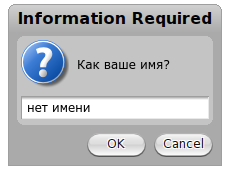
\includegraphics[width=0.8\textwidth]{dialog-ru}}
	%\caption{An input dialog.}\figlabel{dialogName}
	\caption{Диалог ввода.}\figlabel{dialogName}
\end{minipage}
\hfill
\begin{minipage}{0.48\textwidth}
	\vfill
	\centerline{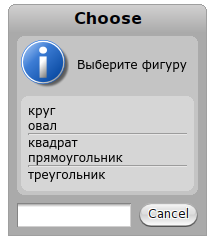
\includegraphics [width=0.8\textwidth]{popup-ru}}
	\vfill
	\vspace{4ex}
	%\caption{Pop-up menu.}\figlabel{popup}
	\caption{Всплывающее меню.}\figlabel{popup}
\end{minipage}
\end{figure}

%To display a popup menu, use one of the various \ct{chooseFrom:} methods (\figref{popup}):
Чтобы отобразить всплывающее меню, используйте один из нескольких методов \ct{chooseFrom:} (\figref{popup}):
\begin{code}{}
UIManager default
	chooseFrom: #('круг' 'овал' 'квадрат' 'прямоугольник' 'треугольник')
	lines: #(2 4) message: 'Выберите фигуру'
\end{code}

%\dothis{Browse the \clsind{UIManager} class and try out some of the interaction methods offered.}
\dothis{Исследуйте класс \clsind{UIManager} и попробуйте некоторые из предоставляемых им методов взаимодействия с пользователем.}

%\begin{figure}[ht]
%	\centerline{\includegraphics[width=5cm]{dialog}}
%	\caption{Dialog displayed by \ct{FillInTheBlank request: 'What''s your name?' initialAnswer: 'no name'}.
%		\figlabel{dialogName}}
%\end{figure}

%To display a pop-up menu, use the \clsind{PopupMenu} class:
%\begin{code}{}
%UIManager default chooseFrom: #('circle' 'oval' 'square' 'rectangle' 'triangle') lines: #(2 4) message: 'Choose a shape'
%\end{code}

%\begin{figure}[ht]
%	\centerline{\includegraphics[width=3cm]{popup}}
%	\caption{PopUp displayed by \ct{PopUpMenu>>>startUpWithCaption:}.}
%\end{figure}

%=================================================================
%\section{Drag-and-drop}
\section{Drag-and-drop}

%Morphic also supports drag-and-drop. Let's examine a simple example with two morphs, a receiver morph and a dropped morph. 
Morphic, кроме прочего, поддерживает и drag-and-drop. Давайте рассмотрим простой пример с двумя морфами, морфом-приёмником и перетаскиваемым морфом.
%The receiver will accept a morph only if the dropped morph matches a given condition: in our example,  the morph should be blue. If it is rejected, the dropped morph decides what to do.
Приёмник примет брошенный морф только если тот соответствует заданному условию: в нашем примере морф должен быть голубым. Если брошенный морф не принят, он сам решает, что делать дальше.

%\dothis{Let's first define the receiver morph:}
\dothis{Давайте сначала определим морф-приёмник:}
%\begin{classdef}{Defining a morph on which we can drop other morphs}
\begin{classdef}{Определяем морф, на который мы сможем перетаскивать другие морфы}
Morph subclass: #ReceiverMorph
	instanceVariableNames: ''
	classVariableNames: ''
	poolDictionaries: ''
	category: 'PBE-Morphic'
\end{classdef}

%\dothis{Now define the initialization method in the usual way:}
\dothis{Определим теперь обычным способом метод инициализации:}
\begin{method}{Initializing \ct{ReceiverMorph}.}
ReceiverMorph>>>initialize
	super initialize.
	color := Color red.
	bounds := 0 @ 0 extent: 200 @ 200
\end{method}

%How do we decide if the receiver morph will accept or repel the dropped morph?
Как же нам решить, должен ли морф-приёмник принять или отклонить брошенный морф?
%In general, both of the morphs will have to agree to the interaction.
В общем случае, оба морфа должны согласиться на это взаимодействие.
%The receiver does this by responding to \mthind{Morph}{wantsDroppedMorph:event:}; the first argument is the dropped morph, and the second the mouse event, so that the receiver can, for example, see if any modifier keys were held down at the time of the drop. 
Приёмник делает это, отвечая на сообщение \mthind{Morph}{wantsDroppedMorph:event:}, где первый аргумент -- это брошенный морф, а второй -- событие мыши, так что получатель может, например, видеть, удерживались ли клавиши-модификаторы, когда морф отпустили.
%The dropped morph is also given the opportunity to check and see if it likes the morph onto which it is being dropped; it is sent the message \ct{wantsToBeDroppedInto:}.  The default implementation of  this method (in class \ct{Morph}) answers \ct{true}.
Брошенному морфу также предоставляется возможность проверить, подходит ли ему морф, над которым его бросили, с помощью сообщения \ct{wantsToBeDroppedInto:}. Реализация по-умолчанию этого метода (в классе \ct{Morph}) возвращает \ct{true}.

%\begin{method}{Accept dropped morphs based on their color.}
\begin{method}{Принимает брошенный морф, основываясь на их цвете.}
ReceiverMorph>>>wantsDroppedMorph: aMorph event: anEvent
	^ aMorph color = Color blue
\end{method}

%What happens to the dropped morph if the receiving morph doesn't want it?  The default behaviour is for it to do nothing, that is, to sit on top of the receiving morph, but without interacting with it.  A more intuitive behavior is for the dropped morph to go back to its original position.  This can be achieved by the receiver answering \ct{true} to the message \mthind{Morph}{repelsMorph:event:} when it doesn't want the dropped morph:
Что случится с брошенным морфом, если принимающий морф не захочет его принять? По-умолчанию он ничего не будет делать. Т.е. он расположится сверху морфа-приёмника, но безо всякого взаимодействия. Но более интуитивное поведение заключалось бы в возвращении брошенного морфа на его исходную позицию. Этого можно достичь, если морф-приёмник ответит \ct{true} на сообщение \mthind{Morph}{repelsMorph:event:} если он не собирается принимать брошенный морф:

\needlines{4}
%\begin{method}{Changing the behaviour of the dropped morph when it is rejected.}
\begin{method}{Изменение поведения брошенного морфа, если он не был принят.}
ReceiverMorph>>>repelsMorph: aMorph event: ev
	^ (self wantsDroppedMorph: aMorph event: ev) not
\end{method}

%That's all we need as far as the receiver is concerned.
Это всё что нам необходимо, касательно приёмника.

%\dothis{Create instances of \clsind{ReceiverMorph} and \clsind{EllipseMorph} in a workspace:}
\dothis{Создайте экземпляры классов \clsind{ReceiverMorph} (приёмник) и \clsind{EllipseMorph} в рабочей области:}
\begin{code}{}
ReceiverMorph new openInWorld.
EllipseMorph new openInWorld.
\end{code}
\noindent
%Try to drag-and-drop the yellow \ct{EllipseMorph} onto the receiver. It will be rejected and sent back to its initial position.
Попробуйте перетащить жёлтый \ct{EllipseMorph} на приёмник. Он не будет принят и вернётся на исходную позицию.

%\dothis{To change this behaviour, change the color of the ellipse morph to \ct{Color blue} using an inspector.  Blue morphs should be accepted by the \ct{ReceiverMorph}.}
\dothis{Чтобы изменить это поведение, смените цвет эллипса с жёлтого на голубой (\ct{Color blue}), используя инспектор.  Голубые морфы должны приниматься экземпляром \ct{ReceiverMorph}.}

%Let's create a specific subclass of \ct{Morph}, named \ct{DroppedMorph}, so we can experiment a bit more:
Давайте создадим подкласс класса \ct{Morph} с именем \ct{DroppedMorph}, чтобы продолжить наш эксперимент:

%\begin{classdef}{Defining a morph we can drag-and-drop onto \ct{ReceiverMorph}}
\begin{classdef}{Определяем морф, который мы сможем перетащить на \ct{ReceiverMorph}}
Morph subclass: #DroppedMorph
	instanceVariableNames: ''
	classVariableNames: ''
	poolDictionaries: ''
	category: 'PBE-Morphic'
\end{classdef}

\needlines{5}
%\begin{method}{Initializing \ct{DroppedMorph}.}
\begin{method}{Инициализация экземпляра \ct{DroppedMorph}.}
DroppedMorph>>>initialize
	super initialize.
	color := Color blue.
	self position: 250@100
\end{method}

%Now we can specify what the dropped morph should do when it is rejected by the receiver; here it will stay attached to the mouse pointer:
Теперь мы можем указать, что брошенный морф должен делать, когда он отклонён приёмником; в данном случае он останется <<приклеенным>> к указателю мыши:
%\begin{method}{Reacting when the morph was dropped but rejected.}
\begin{method}{Реагируем на отказ принять брошенный морф.}
DroppedMorph>>>rejectDropMorphEvent: anEvent
	| h |
	h := anEvent hand.
	WorldState
		addDeferredUIMessage: [h grabMorph: self].
	anEvent wasHandled: true
\end{method}

%Sending the \mthind{MorphicEvent}{hand} message to an event answers the \emph{hand}, an instance of \ct{HandMorph} that represents the mouse pointer and whatever it holds.
Посылка сообщения \mthind{MorphicEvent}{hand} объекту-событию возвращает \emph{указатель} (hand), экземпляр класса \ct{HandMorph}, представляющий указатель мыши и всё, что он удерживает.
%Here we tell the \ct{World} that the hand should grab \ct{self}, the rejected morph.
Здесь мы говорим \ugh{окружению} (\ct{World}), что указатель должен захватить текущий объект \ct{self}, т.е. отклонённый морф.

%\dothis{Create two instances of \ct{DroppedMorph}, and then drag-and-drop them onto the receiver.}
\dothis{Создайте два экземпляра класса \ct{DroppedMorph} и перетащите их на приёмник.}
\begin{code}{}
ReceiverMorph new openInWorld.
(DroppedMorph new color: Color blue) openInWorld.
(DroppedMorph new color: Color green) openInWorld.
\end{code}
\noindent
%The green morph is rejected and therefore stays attached to the mouse pointer.
Зелёный морф будет отклонён и останется прикреплённым к указателю мыши.

%=================================================================
%\section{A complete example}
\section{Законченный пример}

%Let's design a morph to roll a die\footnote{NB: One die, two dice.}. Clicking on it will display the values of all sides of the die in a quick loop, and another click will stop the animation.
Давайте сделаем морф, представляющий собой игральную кость. При клике на нём, быстро чередуясь, будут показываться значения на всех сторонах кости, а повторный клик будет останавливать анимацию.

\begin{figure}[ht]
	\centerline{\includegraphics[scale=0.65]{die}}
	%\caption{The die in Morphic.
	\caption{Игральная кость в Morphic.
		\figlabel{dialogDie}}
\end{figure}

%\dothis{Define the die as a subclass of \clsind{BorderedMorph} instead of \ct{Morph}, because we will make use of the border.}
\dothis{Определите игральную кость как подкласс класса \clsind{BorderedMorph}, а не \ct{Morph}, потому что нам понадобится обрамление.}

\needlines{6}
%\begin{classdef}{Defining the die morph}
\begin{classdef}{Определяем морф, представляющий игральную кость}
BorderedMorph subclass: #DieMorph
	instanceVariableNames: 'faces dieValue isStopped'
	classVariableNames: ''
	poolDictionaries: ''
	category: 'PBE-Morphic'
\end{classdef}

%The instance variable \ct{faces} records the number of faces on the die; we allow dice with up to 9 faces! \ct{dieValue} records the value of the face that is currently displayed, and \ct{isStopped} is true if the die animation has stopped running.
Переменная экземпляра \ct{faces} (грани игральной кости) содержит количество граней на кости. Мы будем допускать не больше девяти граней! Переменная \ct{dieValue} содержит число, которое нанесено на отображаемую в данный момент грань, а переменная \ct{isStopped} определяет, запущена анимация или нет.
%To create a die instance, we define the \ct{faces: n} method on the \emph{class} side of \clsind{DieMorph} to create a new die with \ct{n} faces.
Чтобы создать экземпляр игральной кости с \ct{n} гранями, мы определим метод \ct{faces: n} в \clsind{DieMorph} \emph{на стороне класса}. 
%\begin{method}{Creating a new die with the number of faces we like.}
\begin{method}{Создаём новую игральную кость с нужным нам количеством граней.}
DieMorph class>>>faces: aNumber
	^ self new faces: aNumber
\end{method}

%The \ct{initialize} method is defined on the instance side in the usual way; remember that \ct{new} sends \ct{initialize} to the newly-created instance.
Метод \ct{initialize} определён совершенно обычным образмо на стороне экземпляра (вы ведь помните, что из метода \ct{new} вновь созданному экземпляру посылается сообщение \ct{initialize}).
%\begin{method}{Initializing instances of \ct{DieMorph}.}
\begin{method}{Инициализируем экземпляр класса \ct{DieMorph}.}
DieMorph>>>initialize
	super initialize.
	self extent: 50 @ 50.
	self useGradientFill; borderWidth: 2; useRoundedCorners.
	self setBorderStyle: #complexRaised.
	self fillStyle direction: self extent.
	self color: Color green.
	dieValue := 1.
	faces := 6.
	isStopped := false
\end{method}

%We use a few methods of \ct{BorderedMorph} to give a nice appearance to the die: a thick border with a raised effect, rounded corners, and a color gradient on the visible face.
Мы используем несколько методов класса \ct{BorderedMorph}, чтобы придать красивый вид нашей игральной кости: добавить ей рельефную рамку, скруглённые углы, цветной градиент на видимой грани.
%We define the instance method \ct{faces:} to check for a valid parameter as follows:
Мы определим метод экземпляра \ct{faces:} следующим образом, чтобы проверять преданный параметр:
\begin{method}{Setting the number of faces of the die.}
DieMorph>>>faces: aNumber
	"Устанавливает количество граней"
	(aNumber isInteger
			and: [aNumber > 0]
			and: [aNumber <= 9])
		ifTrue: [faces := aNumber]
\end{method}
\on{Why not make this a pre-condition, \ie an assertion?}

%It may be good to review the order in which the messages are sent when a die is created. For instance, if we start by
Вероятно, будет полезным ещё раз проверить порядок, в котором сообщения будут посылаться вновь созданной игральной кости. Например, если мы начнём с 
%evaluating \ct{DieMorph faces: 9}:
вычисления \ct{DieMorph faces: 9}:
\begin{enumerate}
%	\item The class method \ct{DieMorph class>>>faces:} sends \ct{new} to \ct{DieMorph class}.
	\item Метод класса \ct{DieMorph class>>>faces:} посылает \ct{new} объекту \ct{DieMorph class}.
%	\item The method for \ct{new} (inherited by \ct{DieMorph class} from \ct{Behavior}) creates the new instance and sends it the \ct{initialize} message.
	\item Метод \ct{new} (унаследованный объектом \ct{DieMorph class} от класса \ct{Behavior}) создаёт новый экземпляр и посылает ему сообщение \ct{initialize}.
%	\item The \ct{initialize} method in \ct{DieMorph} sets \ct{faces} to an initial value of 6.
	\item Метод \ct{initialize} в классе \ct{DieMorph} устанавливает начальное значение \ct{faces} равным 6
%	\item \ct{DieMorph class>>>new} returns to the class method \ct{DieMorph class>>>faces:}, which then sends the message \ct{faces: 9} to the new instance.
	\item \ct{DieMorph class>>>new} возвращает управление методу \ct{DieMorph class>>>faces:}, который посылает сообщение \ct{faces: 9} новому экземпляру.
%	\item The instance method \ct{DieMorph>>>faces:} now executes, setting the \ct{faces} instance variable to 9.
	\item Выполняется метод экземпляра \ct{DieMorph>>>faces:}, устанавливающий переменную экземпляра \ct{faces} равной 9.
\end{enumerate}

%Before defining \ct{drawOn:}, we need a few methods to place the dots on the displayed face:
Перед определением метода \ct{drawOn:} нам нужно несколько методов, чтобы расположить точки на отображаемой грани:
%\begin{methods}{Nine methods for placing points on the faces of the die.}
\begin{methods}{Девять методов для расположения точек на гранях игральной кости.}
DieMorph>>>face1
	^{0.5@0.5}
DieMorph>>>face2
	^{0.25@0.25 . 0.75@0.75}
DieMorph>>>face3
	^{0.25@0.25 . 0.75@0.75 . 0.5@0.5}
DieMorph>>>face4
	^{0.25@0.25 . 0.75@0.25 . 0.75@0.75 . 0.25@0.75}
DieMorph>>>face5
	^{0.25@0.25 . 0.75@0.25 . 0.75@0.75 . 0.25@0.75 . 0.5@0.5}
DieMorph>>>face6
	^{0.25@0.25 . 0.75@0.25 . 0.75@0.75 . 0.25@0.75 . 0.25@0.5 . 0.75@0.5}
DieMorph>>>face7
	^{0.25@0.25 . 0.75@0.25 . 0.75@0.75 . 0.25@0.75 . 0.25@0.5 . 0.75@0.5 . 0.5@0.5}
DieMorph >>>face8
	^{0.25@0.25 . 0.75@0.25 . 0.75@0.75 . 0.25@0.75 . 0.25@0.5 . 0.75@0.5 . 0.5@0.5 . 0.5@0.25}
DieMorph >>>face9
	^{0.25@0.25 . 0.75@0.25 . 0.75@0.75 . 0.25@0.75 . 0.25@0.5 . 0.75@0.5 . 0.5@0.5 . 0.5@0.25 . 0.5@0.75}
\end{methods}
\on{kind of ugly boilerplate code -- should be a nice way to map these more elegantly to coordinates.}

%These methods define collections of the coordinates of dots for each face. The coordinates are in a square of size $1\times1$; we will simply need to scale them to place the actual dots.
Эти методы определяют коллекции координат точек на каждой грани. Т.к. координаты заданы в квадратной области размером $1\times1$, нам потребуется только масштабировать их, чтобы разместить реальные точки.

%The \ct{drawOn:} method does two things: it draws the die background with the \ct{super}-send, and then draws the dots.
Метод \ct{drawOn:} выполняет две вещи: рисует фон игральной кости с помощью вызова метода суперкласса, а затем рисует точки.
\begin{method}{Рисуем морф игральной кости.}
DieMorph>>>drawOn: aCanvas
	super drawOn: aCanvas.
	(self perform: ('face' , dieValue asString) asSymbol)
		do: [:aPoint | self drawDotOn: aCanvas at: aPoint]
\end{method}

%The second part of this method uses the reflective capacities of \st.
Вторая часть этого метода использует рефлексивные возможности \st.
%Drawing the dots of a face is a simple matter of iterating over the collection given by the \ct{faceX} method for that face, sending the \ct{drawDotOn:at:} message for each coordinate. To call the correct \ct{faceX} method, we use the \mthind{Object}{perform:} method which sends a message built from a string, here \lct{('face', dieValue asString) asSymbol}. You will encounter this use of \ct{perform:} quite regularly.
Рисование точек на грани --- это просто вопрос итерации по коллекции, возвращаемой методом \ct{faceX} для данной грани, и посылка сообщения \ct{drawDotOn:at:} каждой координате. Чтобы вызвать нужный метод \ct{faceX}, мы используем метод \mthind{Object}{perform:}, который посылает сообщение, имя которого получается из строки \lct{('face', dieValue asString) asSymbol}. С таким использованием метода \ct{perform:} вы будете сталкиваться практически постоянно.
\index{reflection}
%\begin{method}{Drawing a single dot on a face.}
\begin{method}{Рисуем одну точку на грани.}
DieMorph>>>drawDotOn: aCanvas at: aPoint
	aCanvas
		fillOval: (Rectangle
			center: self position + (self extent * aPoint)
			extent: self extent / 6)
		color: Color black
\end{method}
\ew{I would not use reflection to call faceX on p.234. A statically filled Dictionary would be more appropriate. Get the point set with "MyDict at: X".}

%Since the coordinates are normalized to the $[0{:}1]$ interval, we scale them to the dimensions of our die: \ct{self extent * aPoint}.
Т.к координаты нормированы по отрезку $[0{:}1]$, мы можем масштабировать их до размеров нашей игральной кости: \ct{self extent * aPoint}

%\dothis{We can already create a die instance from a workspace:}
\dothis{Мы уже можем создать экземпляр игральной кости из рабочей области:}
\begin{code}{}
(DieMorph faces: 6) openInWorld.
\end{code}

%To change the displayed face, we create an accessor that we can use as \ct{myDie dieValue: 4}:
Чтобы изменить отображаемую грань, мы создадим аксессор, который будем использовать как \ct{myDie dieValue: 4}:
%\begin{method}{Setting the current value of the die.}
\begin{method}{Установка текущего значения игральной кости.}
DieMorph>>>dieValue: aNumber
	(aNumber isInteger
			and: [aNumber > 0]
			and: [aNumber <= faces])
		ifTrue:
			[dieValue := aNumber.
			self changed]
\end{method}

%Now we will use the animation system to show quickly all the faces:
А теперь используем анимацию для быстрого показа всех граней:
\needlines{3}
\index{Morphic!animation}
%\begin{methods}{Animating the die.}
\begin{methods}{Анимирование игральной кости.}
DieMorph>>>stepTime
	^ 100

DieMorph>>>step
	isStopped ifFalse: [self dieValue: (1 to: faces) atRandom]
\end{methods}
%Now the die is rolling!
Теперь наша игральная кость <<катится>>!

%To start or stop the animation by clicking, we will use what we learned previously about mouse events.
Чтобы запустить или остановить анимацию с помощью клика, мы используем полученные ранее знания о событиях мыши.
%First, activate the reception of mouse events:
Для начала, сделаем возможным приём таких событий.

%\begin{methods}{Handling mouse clicks to start and stop the animation.}
\begin{methods}{Обрабатываем клики мыши, чтобы запускать и останавливать анимацию.}
DieMorph>>>handlesMouseDown: anEvent
	^ true

DieMorph>>>mouseDown: anEvent
	anEvent redButtonPressed
		ifTrue: [isStopped := isStopped not]
\end{methods}
%Now the die will roll or stop rolling when we click on it.
Теперь игральная кость будет <<катиться>> когда мы кликнем на ней.

% That's all for the essentials of Morphic!

% Most of the work on \ct{DieMorph} was done with an instance of it living in the environment; this is quite nice when to tweak programs.

%=================================================================
%\section{More about the canvas}
\section{Ещё о канве}

%The \ct{drawOn:} method has an instance of \clsindmain{Canvas} as its sole argument;
Метод \ct{drawOn:} принимает экземпляр класса \clsindmain{Canvas} (Канва) в качестве единственного своего аргумента.
%the canvas is the area on which the morph draws itself.
Канва --- это область, на которой морф отрисовывает себя.
%By using the graphics methods of the canvas you are free to give the appearance you want to a morph.
Используя графические методы канвы вы можете придать своему морфу совершенно произвольный вид.
%If you browse the inheritance hierarchy of the \ct{Canvas} class, you will see that it has several variants.
Если вы посмотрите на иерархию наследования класса \ct{Canvas}, вы увидите, что канва имеет несколько разновидностей.
%The default variant of \ct{Canvas} is \clsind{FormCanvas}; you will find the key graphics methods in \ct{Canvas} and \ct{FormCanvas}.
Используемый по-умолчанию вид канвы --- это \clsind{FormCanvas}, здесь (и в классе \ct{Canvas}) вы найдёте ключевые графические методы.
%These methods can draw points, lines, polygons, rectangles, ellipses, text, and images with rotation and scaling.
Эти методы могут рисовать точки, линии, многоугольники, прямоугольники, текст и изображения с вращением и масштабированием.

%It is also possible to use other kinds of canvas, to obtain transparent morphs, more graphics methods, antialiasing, and so on.
Возможно использовать другие разновидности канвы, чтобы получить прозрачные морфы, больше графических методов, сглаживание и т.д.
%To use these features you will need an \clsind{AlphaBlendingCanvas} or a \clsind{BalloonCanvas}.
Чтобы использовать эти возможности, вам потребуются \clsind{AlphaBlendingCanvas} или \clsind{BalloonCanvas}.
%But how can you obtain such a canvas in a \ct{drawOn:} method, when \ct{drawOn:} receives an instance of \ct{FormCanvas} as its argument?
Но как получить нужную канву в методе \ct{drawOn:}, если он уже получает экземпляр класса \ct{FormCanvas} в качестве аргумента?
%Fortunately, you can transform one kind of canvas into another.
К счастью, вы можете преобразовать один вид канвы в другой.

%\dothis{To use a canvas with a 0.5 alpha-transparency in \ct{DieMorph}, redefine \ct{drawOn:} like this:}
\dothis{Чтобы использовать канву с альфа-прозрачностью равной 0.5 в \ct{DieMorph}, переопределите метод \ct{drawOn:} следующим образом:}
\needlines{7}
%\begin{method}{Drawing a translucent die.}
\begin{method}{Рисуем полупрозрачную игральную кость.}
DieMorph>>>drawOn: aCanvas
	| theCanvas |
	theCanvas := aCanvas asAlphaBlendingCanvas: 0.5.
	super drawOn: theCanvas.
	(self perform: ('face' , dieValue asString) asSymbol)
		do: [:aPoint | self drawDotOn: theCanvas at: aPoint]
\end{method}
\noindent
%That's all you need to do!
Это всё, что вам нужно сделать!

\begin{figure}[ht]
	\centerline{\includegraphics[scale=0.7]{multiMorphs}}
	%\caption{The die displayed with alpha-transparency.
	\caption{Игральная кость, отображаемая с альфа-прозрачностью.
		\figlabel{multiMorphs}}
\end{figure}

% ON: This appears to be broken:

%If you're curious, have a look at the \mthind{Canvas}{asAlphaBlendingCanvas:} method.
%You can also get antialiasing by using \clsind{BalloonCanvas} and transforming the die drawing methods as shown in \mthsref{aadie}.

%\needlines{6}
%\begin{methods}[aadie]{Drawing an antialiased die.}
%DieMorph>>>drawOn: aCanvas
%	| theCanvas |
%	theCanvas := aCanvas asBalloonCanvas aaLevel: 3.
%	super drawOn: aCanvas.
%	(self perform: ('face' , dieValue asString) asSymbol)
%		do: [:aPoint | self drawDotOn: theCanvas at: aPoint]

%DieMorph>>>drawDotOn: aCanvas at: aPoint
%	aCanvas
%		drawOval: (Rectangle
%			center: self position + (self extent * aPoint)
%			extent: self extent / 6)
%		color: Color black
%		borderWidth: 0
%		borderColor: Color transparent
%\end{methods}

%=================================================================
%\section{Chapter summary}
\section{Итоги главы}

%Morphic is a graphical framework in which graphical interface elements can be dynamically composed.
Морфик --- это графический фреймворк, в котором элементы графического элемента могут компоноваться динамическим образом.

\begin{itemize}
%  \item You can convert an object into a morph and display that morph on the screen by sending it the messages \ct{asMorph openInWorld}.
  \item Вы можете преобразовать объект в морф и отобразить его на экране, послав этому объекту сообщения \ct{asMorph openInWorld}.
%  \item You can manipulate a morph by \metaclick{ing} on it and using the handles that appear. (Handles have help balloons that explain what they do.)
  \item Вы можете манипулировать морфом, сделав на нём \metaclick, и используя появившиеся кнопки, к каждой из которых прилагается появляющееся облачко с подсказкой.
%  \item You can compose morphs by embedding one onto another, either by drag and drop or by sending the message \ct{addMorph:}.
  \item Вы можете компоновать морфы, встраивая один в другой, либо с помощью drag-and-drop'а, либо послав сообщение \ct{addMorph:}.
%  \item You can subclass an existing morph class and redefine key methods, like \ct{initialize} and \ct{drawOn:}.
  \item Вы можете наследоваться от существующих классов морфов и переопределять их ключевые методы, как, например, \ct{initialize} и \ct{drawOn:}.
%  \item You can control how a morph reacts to mouse and keyboard events by redefining the methods \ct{handlesMouseDown:}, \ct{handlesMouseOver:}, \etc
  \item Вы можете контролировать то, каким образом морф реагирует на события мыши и клавиатуры, переопределяя методы \ct{handlesMouseDown:}, \ct{handlesMouseOver:}, \etc
%  \item You can animate a morph by defining the methods \ct{step} (what to do) and \ct{stepTime} (the number of milliseconds between steps).
  \item Вы можете анимировать морф, определив методы \ct{step}, определяющий, что делать на данном шаге анимации, и \ct{stepTime}, определяющий количество миллисекунд между шагами.
%  \item Various pre-defined morphs, like \ct{PopUpMenu} and \ct{FillInTheBlank}, are available for interacting with users.
  \item Имеется большой набор морфов, таких, как \ct{PopUpMenu} и \ct{FillInTheBlank}, предназначенных для взаимодействия с пользователем.
\end{itemize}

%=================================================================
\ifx\wholebook\relax\else\end{document}\fi
%=================================================================

%-----------------------------------------------------------------
